\chapter{The CMS Experiment}

In the previous chapter we summarized the theoretical underpinnings of modern
particle physics, and discussed possible extensions that point towards
future research. We now turn our attention to the machines that make such
research possible. The Large Hadron Collider (LHC) is the largest
particle collider ever built, smashing protons together at record energies.
On it are located four major experiments, designed to record electrical
snapshots of the collisions and allow physicists to reconstruct the details
of each event. Sec.~\ref{sec:lhc} describes the design and operation of the LHC,
and Sec.~\ref{sec:cms_det} introduces the Compact Muon Solenoid (CMS) experiment,
one of the four at the LHC and the one used for the analysis in this dissertation.

\section{The Large Hadron Collider}
\label{sec:lhc}

Underneath the French-Swiss border near the city of Geneva lies the LHC, the world's largest 
proton collider. With a circumference of 26.7 kilometers and depth of up to 175
meters below ground, it is designed to accelerate protons to an energy of 7\TeV, over
7,000 times their rest mass (and corresponding to a speed 
99.9999991\% the speed of light). Utilizing the tunnel of the older Large Electron--Positron
collider (LEP) at CERN, it was constructed to supersede the Tevatron at Fermilab, which
accelerated protons to 1\TeV.

What was the motivation for such a machine? The LEP collider, which accelerated electrons
and positrons to up to 209\GeV, had allowed for precise measurements of many SM quantities
inclusing the $W$ and $Z$ masses, but was not able to find definitive proof of a Higgs boson
or any evidence for BSM physics. Similarly, the Tevatron had discovered the top quark
and made many measurements but failed to find evidence of the Higgs or new physics. Physicists
thus sought a next-generation machine that could find these things.

\begin{figure}[t]
  \begin{center}
    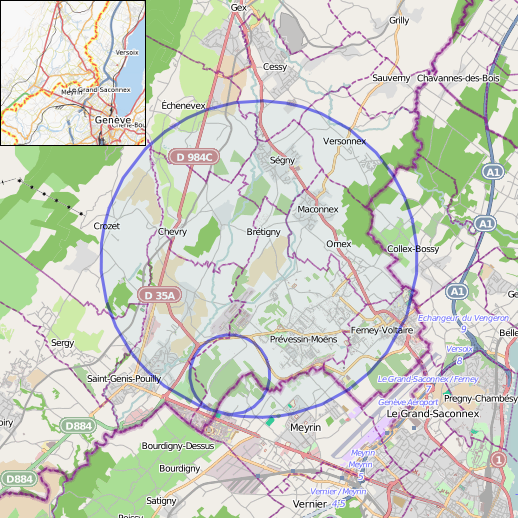
\includegraphics[width=0.39\textwidth]{figs/cms/lhc_osm.png}
    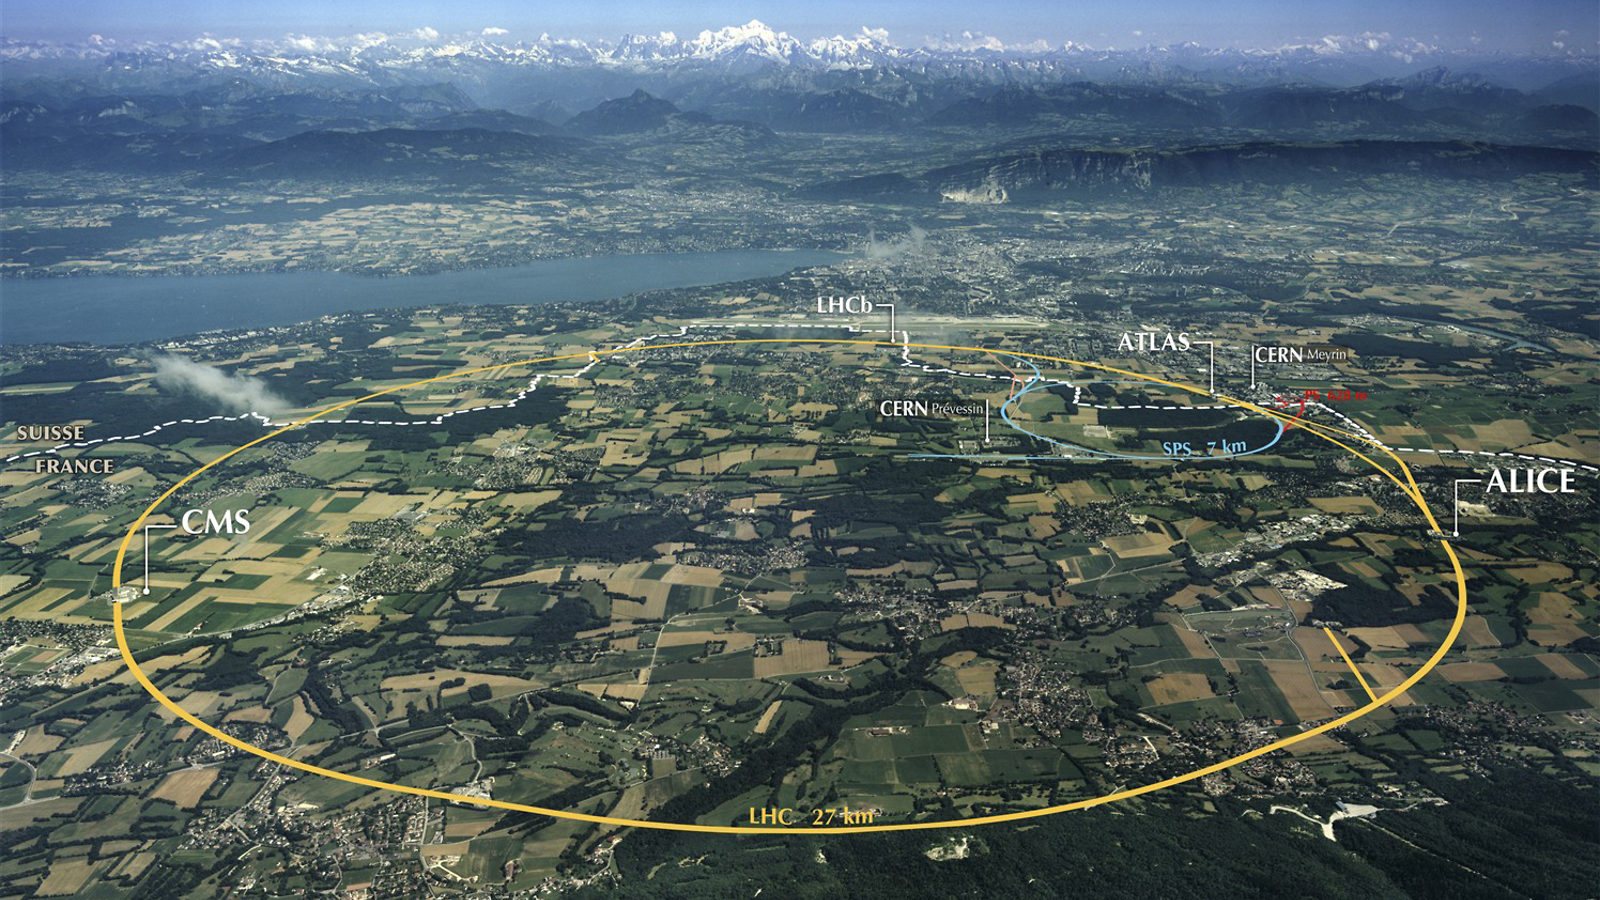
\includegraphics[width=0.59\textwidth]{figs/cms/lhc_photo.jpg} 
    \caption{(left) The SPS and LHC overlaid on a map of the Franco-Swiss border near Geneva. The diameter of
      the LHC is 8.5 km (5.3 miles). (right) The LHC, the four major experiments, and CERN's campus 
      overlaid on a photo of the Geneva area, looking southeast. Lake Geneva and the French Alps can
      be seen in the background. (Images from \cite{lhc_map,lhc_photo})
            }
    \label{fig:lhc}
  \end{center}
\end{figure}

Since the Higgs and potential new physics were at energy scales above the reach of
present experiments, a higher energy collider was needed. 
Circular lepton colliders like LEP
are limited in energy, as the energy radiated by an accelerating charged particle falls as 
$1/m^4r^2$, and so the size of the necessary electron collider would be prohibitive.
The much heavier proton is far easier to accelerate to high energies, and an accelerator
in the pre-existing LEP tunnel was sufficient to achieve the necessary energies
(and additionally, cost-effective).
The downside is that collisions of composite particles like protons are messy, and
the actual parton collision energy is indeterminate. However, the LHC was meant do be a 
``discovery machine'', so probing a wide range of collision energies was desirable.
For precision studies of any interesting physics uncovered by the LHC, a future
linear $e^+e^-$ collider would be a good option.

From these considerations, the particle physics community 
decided on a $pp$ collider built in the LEP tunnel,
and construction on the LHC began in 1998. A map of its location can be seen in
Fig.~\ref{fig:lhc}. It sits in a tunnel between 50 and 175 meters underneath
the suburbs of Geneva, Switzerland, straddling the France-Switzerland border.
To the west are the Jura mountains, and to the east Lake Geneva. The CERN
campus is on the south end.

\begin{figure}[t]
  \begin{center}
    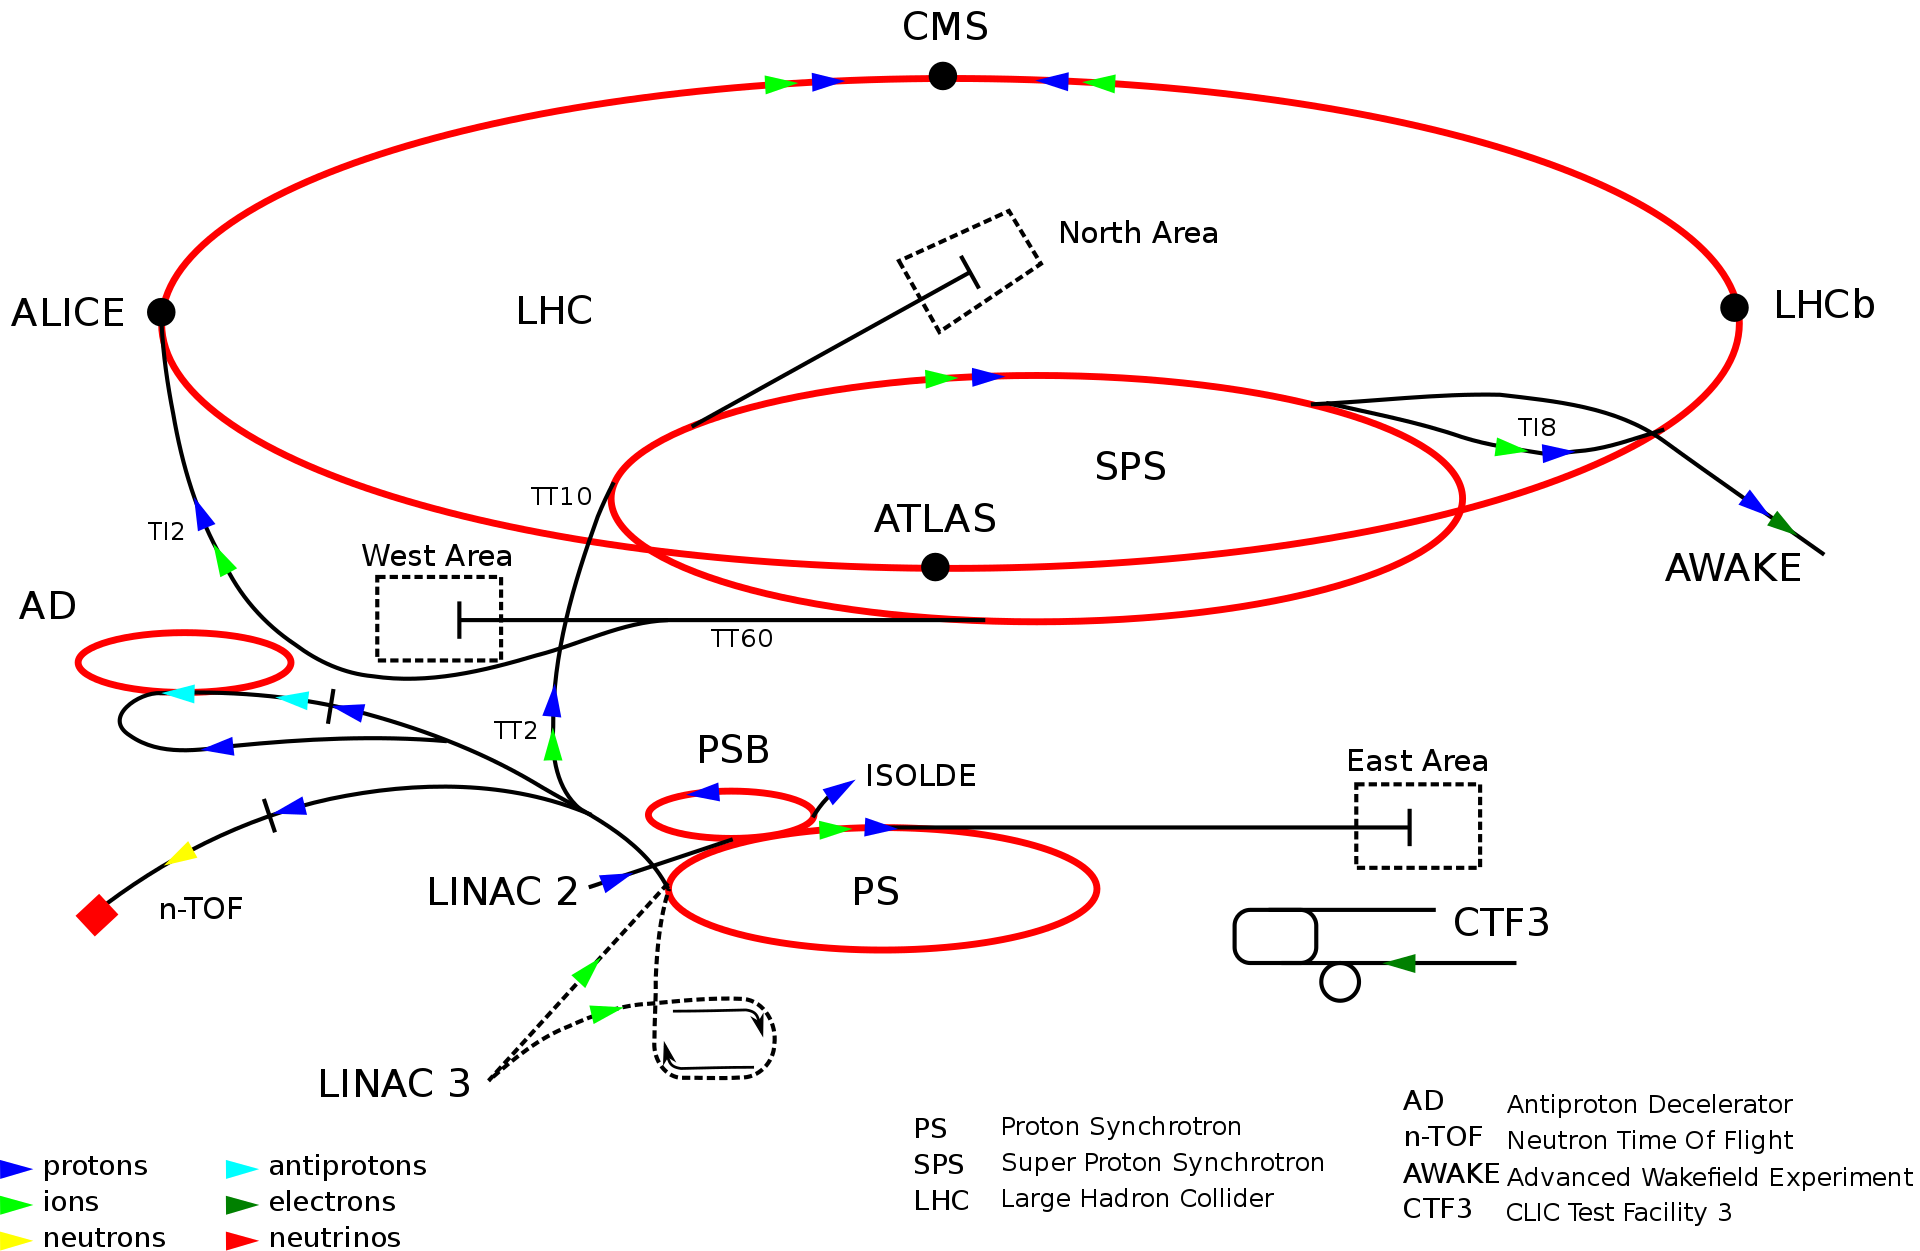
\includegraphics[width=0.60\textwidth]{figs/cms/accelerator_complex.png}
    \caption{The CERN accelerator complex. Protons originate in the LINAC 2 where they are 
      injected at 50\MeV into the PSB. The PSB, PS, and SPS subsequently accelerate them
      to 1.4\GeV, 26\GeV, and 450\GeV, respectively, before they enter the LHC where they
      reach up to 6.5\TeV. (Image from~\cite{accelerator_complex})
            }
    \label{fig:cern_accelerator_complex}
  \end{center}
\end{figure}

Before entering the main ring, the protons progress through a series of
increasingly large accelerators. The steps in the chain are as follows;
the CERN accelerator complex is
illustrated in Fig.~\ref{fig:cern_accelerator_complex}. 
\begin{itemize}\setlength\itemsep{-1mm}
\item The protons begin as nuclei in hydrogren gas, and electric fields are used to strip the electrons away.
\item The bare protons are fed into the linear LINAC 2 accelerator, where
they are boosted to 50\MeV kinetic energy and injected into the 160 meter
Proton Synchrotron Booster (PSB).
\item The PSB accelerates the protons to 1.4\GeV and feeds them into the
628 meter Proton Synchrotron (PS).
\item The PS accelerates them to 26\GeV and injects them into the
6.9 kilometer Super Proton Synchrotron (SPS).
\item The SPS accelerates them to 450\GeV before finally injecting
them into the main 26.7 kilometer LHC ring (it inserts two beams, traveling
in opposite directions)
\item Over a period of around 20 minutes, the LHC accelerates the protons
to 6.5\TeV (this is the present maximum; the LHC is designed to eventually
go to 7\TeV).
\end{itemize}

In order to steer the beams in a circle, the LHC makes use of powerful superconducting
magnets. Dipole magnets are used as the main steering mechanism. From the formula 
for a relativistic charged particle in a uniform magnetic field, the necessary average
magnetic field is $B=\gamma m\beta/qR=5.1~\mrm{T}$. However, the magnets are not all the
way around the ring so the peak dipole magnetic field is 7.74 T. In addition to the dipole magnets,
quadrupole magnets are used for beam focusing, and higher multipole magnets are used for finer
corrections. In total there are nearly 10,000 individual magnets. In order to maintain a such a
strong field, the superconducting magnets operate at a temperature of only 1.9 K, achieved
using 96 tons of superfluid helium~\cite{lhc_guide}.

Magnets can only steer the beam, not increase its energy. In order to perform
the acceleration from 450\GeV to 6.5\TeV, the LHC makes use of 8 radio-frequency
(RF) cavities per direction that produce an oscillating electric field at a frequency of
400 MHz. This naturally produces a beam of ``bunches'', spaced 25 ns apart:
the electric fields boost the protons, and the gradient of the field is
constructed in such a way that any protons that arrive early or late
recieve a slightly different kick, pushing them back towards the bunch
center.

Together, the magnetic and electric fields produce two counter-rotating
beams of 6.5\TeV protons, organized into bunches 25 ns apart (corresponding
to around 7.5 m of spatial separation). There are about
$1.2\times10^{11}$ protons per bunch, and up to 2808 bunches per beam, giving
$3.4\times10^{14}$ protons in each beam. At 6.5\TeV each, the total kinetic energy
in both beams together is over 700 million joules, equivalent
to a Boeing 737 traveling at 200 mph!

The ``collision rate'' at colliders is measured with a quantity known as instantaneous
luminosity, defined by the rate $N$ of a given type of interaction with cross section (roughly, likelihood
of interaction) $\sigma$ as $\mathcal{L}=N\sigma$. This luminosity is a function of
the bunch crossing rate (at the LHC, once every 25 ns), the number of protons
per bunch, and the effective area of the beam (i.e., how tightly packed
the protons in the beam are). The LHC can reach an instantaneous luminosity of
around $2\times10^{34}~\mrm{cm}^{-2}\mrm{s}^{-1}$.

The total proton-proton inelastic cross section is measured to be around 78 mb~\cite{ATLAS:ppxsec}.
Multiplying by the LHC instantaneous luminosity, that means we expect
1.5 billion inelastic collisions per second, or around 40 per bunch crossing.
Most of these will be relatively uninteresting, and a major challenge in analyzing experimental
data is disentagling the interesting event from the $\sim40$ other interactions
(referred to as \textit{pileup} interactions).

The LHC began beam operations in September 2008. Just nine days after the
first beams circulated, an electrical fault led to the loss of
six tons of liquid helium, causing a magnet quench and an explosion
that damaged 53 magnets~\cite{LHC_incident}. This delayed the start of physics by a year until
November 2009, and limited the collision energy in the LHC's first run to 8\TeV.
This Run 1 lasted through the beginning of 2013, before a two year shutdown
and the start of 13\TeV collisions in Run 2 in 2015.

The LHC steers the counter-rotating beams to collide at four pre-defined
experimental interaction points, corresponding to the ATLAS, ALICE,
CMS, and LHCb experiments (illustrated in Figs.~\ref{fig:lhc} (right)
and \ref{fig:cern_accelerator_complex}).
ALICE is optimized to study collisions of Pb nuclei
(another capability of the LHC, and the reason for the use of 
``hadron collider'' instead of ``proton collider''), which
produce quark--gluon plasma. LHCb is an asymmetric forward
detector meant to study processes involving $B$ hadrons.
CMS and ATLAS are both general-purpose hermetic detectors,
meant to study a wide range of physics. 
We now turn our attention to the CMS experiment, which was used
to collect the data utilized in the present analysis.


\section{The CMS detector}
\label{sec:cms_det}

The Compact Muon Solenoid (CMS) detector is one of two general-purpose detectors
at the LHC, designed to capture the details of proton-proton collisions
as completely as possible in order to study the SM and search for any signs
of physics beyond the SM.

CMS is 21 meters long and 15 meters in diameter (relatively ``compact'', compared
to ATLAS). It is built around a central solenoidal magnet, which
provides a powerful magnetic field that bends the trajectories of charged
particles. The detector consists of various layers of sub-detectors and components,
illustrated in the cutaway diagram in Fig.~\ref{fig:cms_diagram}. The layers,
working from the inside out, are: the beampipe; silicon tracker;
electromagnetic calorimeter; hadronic calorimeter; magnet; muon detectors;
and steel return yokes (these last two are interspersed in alternating layers).
Moreover, these components are organized into a central cylindrical barrel,
providing coverage out to roughly 25$^\circ$ from the beamline,
and two circular endcaps that can be pulled away for access to the detector.
Photos of an opened CMS (i.e. with the endcaps pulled away) are shown in 
Fig.~\ref{fig:cms_photos}.

\begin{figure}[t]
  \begin{center}
    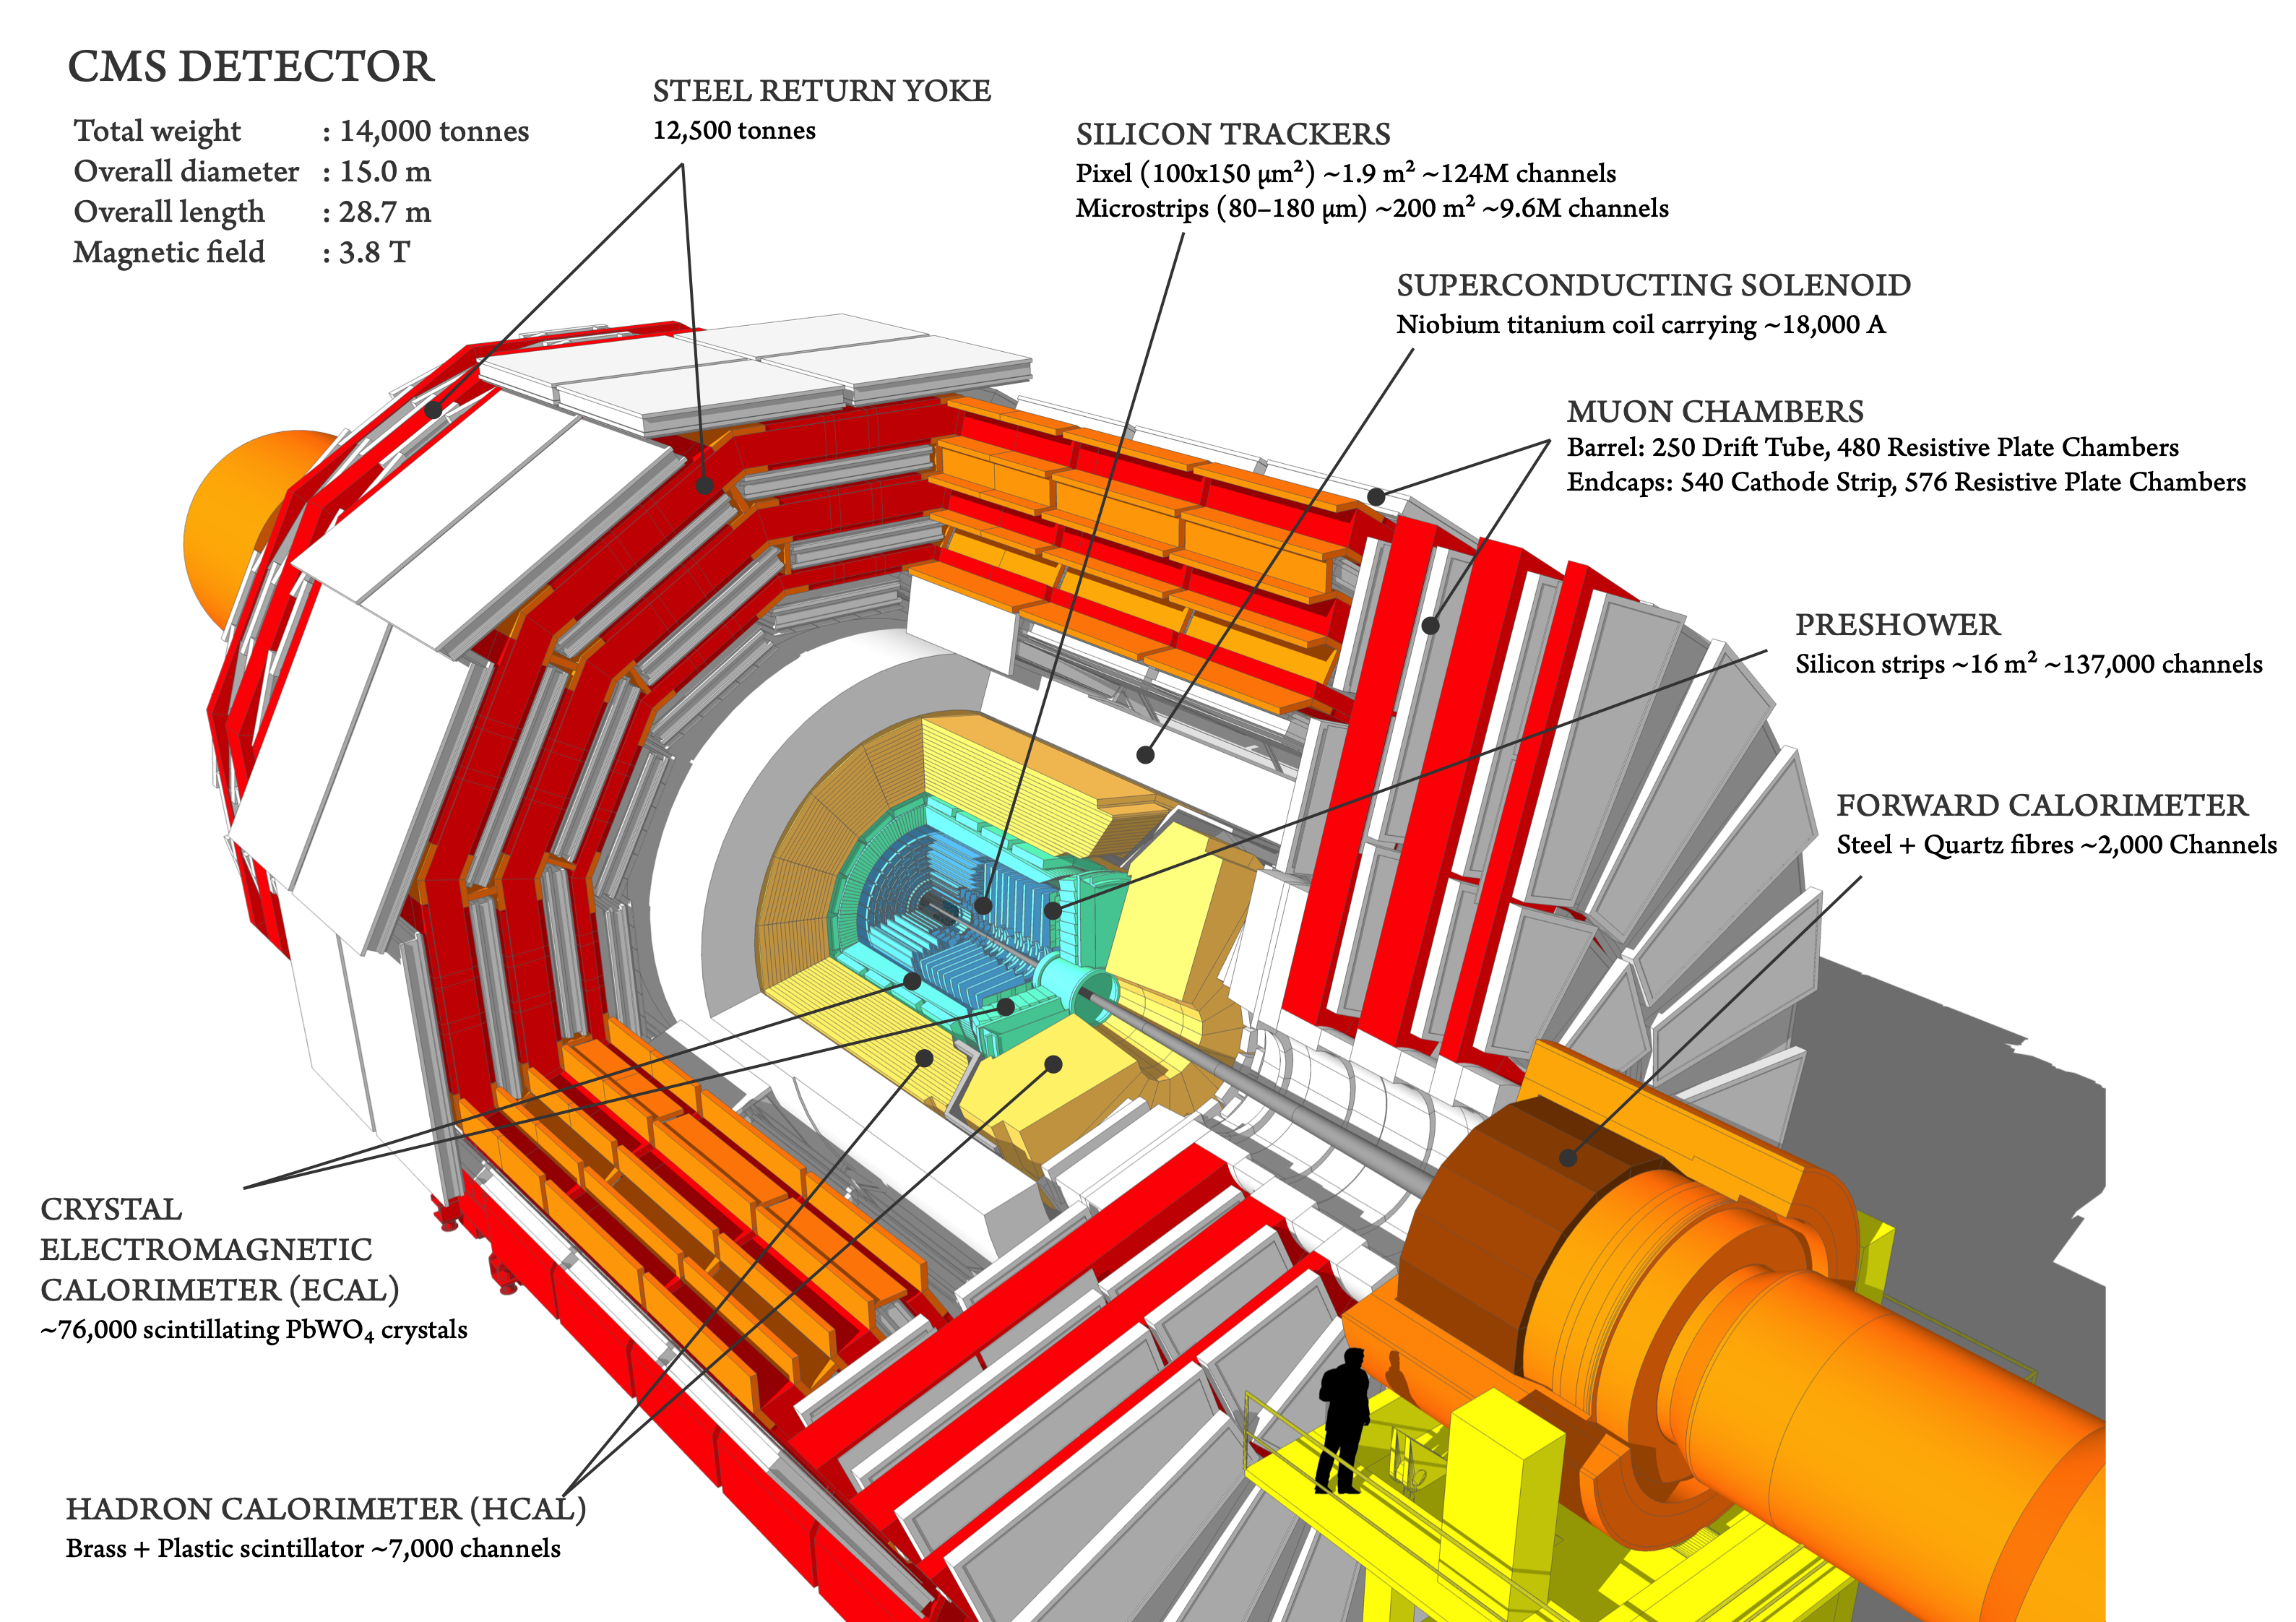
\includegraphics[width=0.99\textwidth]{figs/cms/cms_diagram.png}
    \caption{Cutaway illustration of the CMS detector. Note the outline
      of a human in the lower right for scale. (Image from~\cite{cms_vis})
            }
    \label{fig:cms_diagram}
  \end{center}
\end{figure}

\begin{figure}[t]
  \begin{center}
    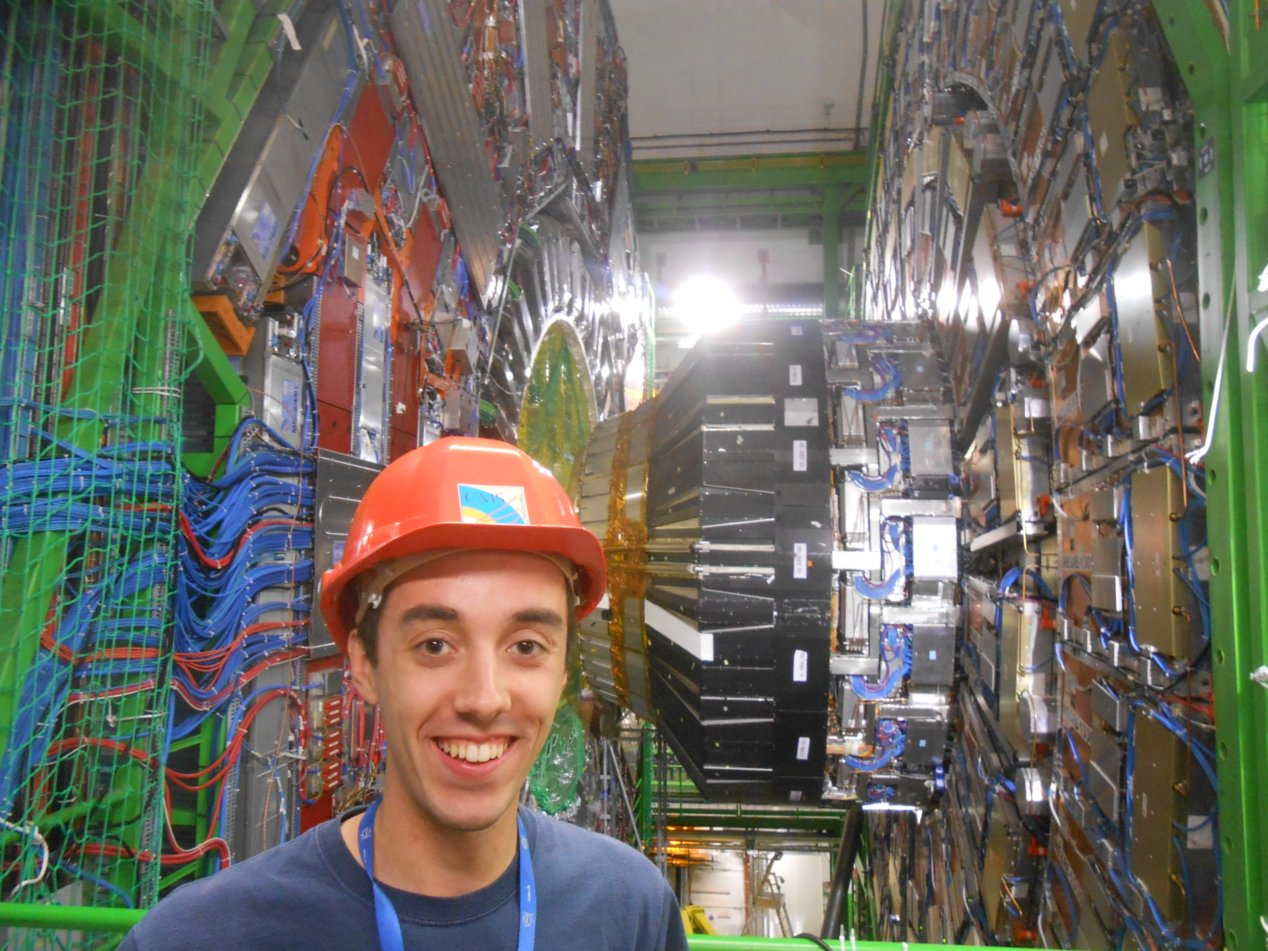
\includegraphics[width=0.45\textwidth]{figs/cms/bennett.jpg}
    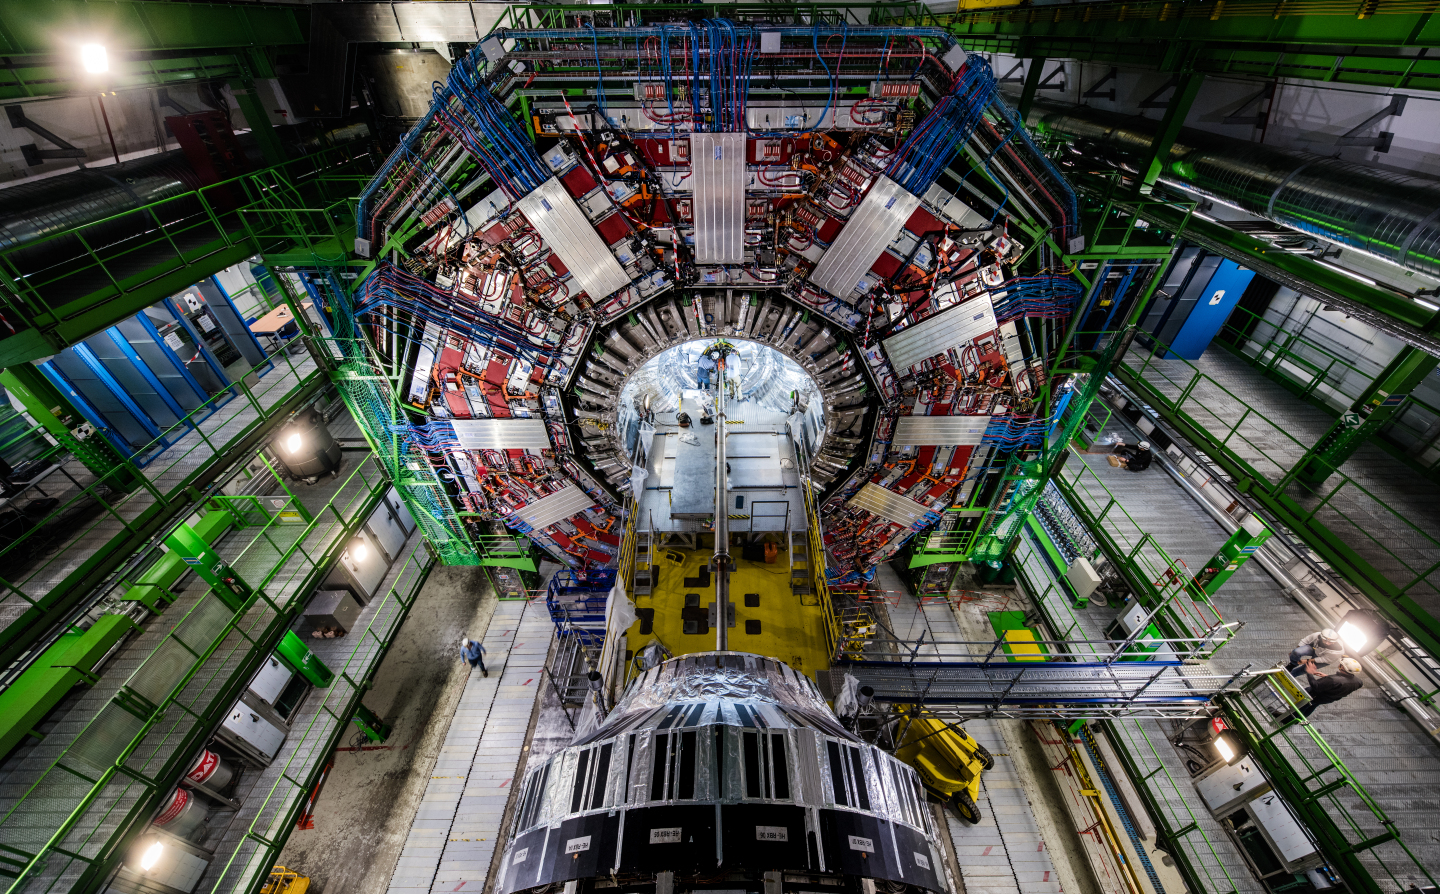
\includegraphics[width=0.54\textwidth]{figs/cms/cms_photo.jpg}
    \caption{(left) The author next to an opened CMS detector in summer 2014.
      On the right side is the muon endcap detector, with the endcap hadronic calorimeter
      protruding. On the left is the barrel, with the muon detectors and iron yokes
      on the outside, and the magnet forming the inner ring.
      (right) A broader view of the opened CMS detector, during the installation
      of the new Phase-1 Upgrade pixel detector in 2017. Note the technicians
      inside the barrel for scale. (Image via Maximilien Brice, CERN)
            }
    \label{fig:cms_photos}
  \end{center}
\end{figure}

We now go through each of the components and briefly describe their design and operation.
More detailed accounts and the full technical details can be found in the CMS Technical
Design Reports (volume I contains detector performace and software~\cite{CMS:tdr_i}, and
volume II describes physics performance~\cite{CMS:tdr_ii}. There are also more recent reports
describing various detector upgrades).

First, a word on coordinates and notation (used in this chapter and throughout this
dissertation): the standard CMS coordinate system is centered on the nominal collision
point, with the $x$ axis pointing radially inward toward the center of the LHC, the
$y$ axis pointing vertically upward, and the $z$ axis pointing along the beamline,
counter-clockwise if looking at the LHC from above. The coordinate $r$ refers to the 
cylindrical radius $r=\sqrt{x^2+y^2}$, and $\phi$ the azimuthal angle $\tan(\phi)=y/x$.
Instead of the polar angle $\theta=\tan^{-1}(r/z)$, particle physicists generally use
psudorapidity $\eta=-\log(\tan(\theta/2))$. The reason is that for relativistic
particles, $\eta$ is a very good approximation of rapidity, and differences in
rapidity are invariant under Lorentz boosts along the $z$ axis. A pseudorapity
of 0 is central (i.e. orthogonal to the beamline), and a pseudorapidity high
in absolute value indicates something nearly parallel to the beamline.
A subscript T on a quantity (e.g. \pt)
indicates the transverse (i.e. $xy$) component.

\subsection{Magnet and return yoke}

The core of CMS is a large solenoid designed to produce a strong magnetic field. Charged
particle trajectories are curved by this field, allowing reconsruction of their momenta
(the radius of curvature is given by $R=\pt/qB$).
The solenoid is 13 meters long and has an inner radius of around 3 meters, making
it the largest solenoidal magnet ever built. The coils are made of superconducting
niobium-titanium, and carry a current of 18,160 A to produce a magnetic field of 3.8 T.

Outside of the magnet coils are three layers of steel (called the ``return yoke''),
which provide support and guide 
the exterior return field (to limit the field strength outside of the physical
detector). A map of the magnetic field magnitude in a cross-sectional
plane of CMS is shown in Fig.~\ref{fig:cms_bfield}. The central 13 m $\times$ 6 m
core is visible, along with the layers of steel return yoke that carry most of the
exterior field. Outside of these structures, the field is relatively small.

\begin{figure}[t]
  \begin{center}
    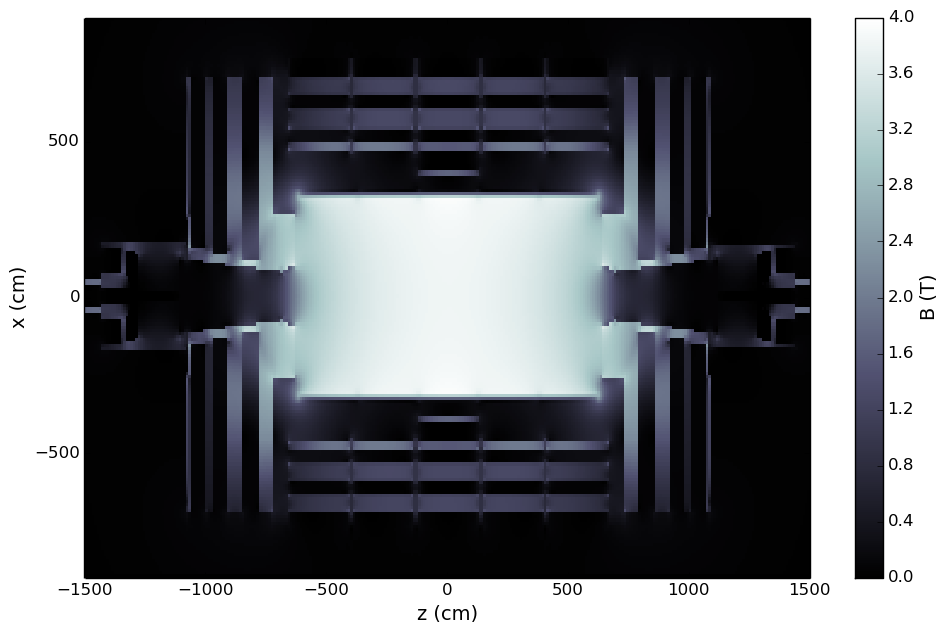
\includegraphics[width=0.60\textwidth]{figs/cms/cms_bfield_coarse.png}
    \caption{Map of the CMS magnetic field magnitude in an $rz$ cross-sectional plane.
      The magnitude is a roughly constant 3.8 T in the core inside the magnet coils, and weaker outside.
      The steel return yokes that carry back most of the magnetic flux are visible.
            }
    \label{fig:cms_bfield}
  \end{center}
\end{figure}

\subsection{Tracker}

The innermost detector, just outside of the beampipe and inside of the calorimeters and magnet,
is the silicon tracking detector. The aim of this detector is to accurately reconstruct the curved
trajectories of charged particles in order to reconstruct their momenta. 

A central challenge in the design of this detector is the radiation level so close to the beam: 
at 10 cm from the beampipe, the incident particle flux is around 10 million per cm$^2$ per second.
Hence, the detector must be radiation-hard. Additionally, material budget should remain
low so as to minimally affect the trajectories of through-going particles, and the detector
should give high spatial resolution and have fast response time, to allow accurate and timely
reconstruction of particle tracks.

From these considerations, a silicon detector was chosen, as silicon is relatively resilient
to radiation and has a fast response time. The detector works by reverse biasing narrow
strips of silicon; throughgoing charged particles then ionize the atoms to create
electron-hole pairs, which can be collected via an voltage gradient and detected
as a small electrical pulse.

\begin{figure}[t]
  \begin{center}
    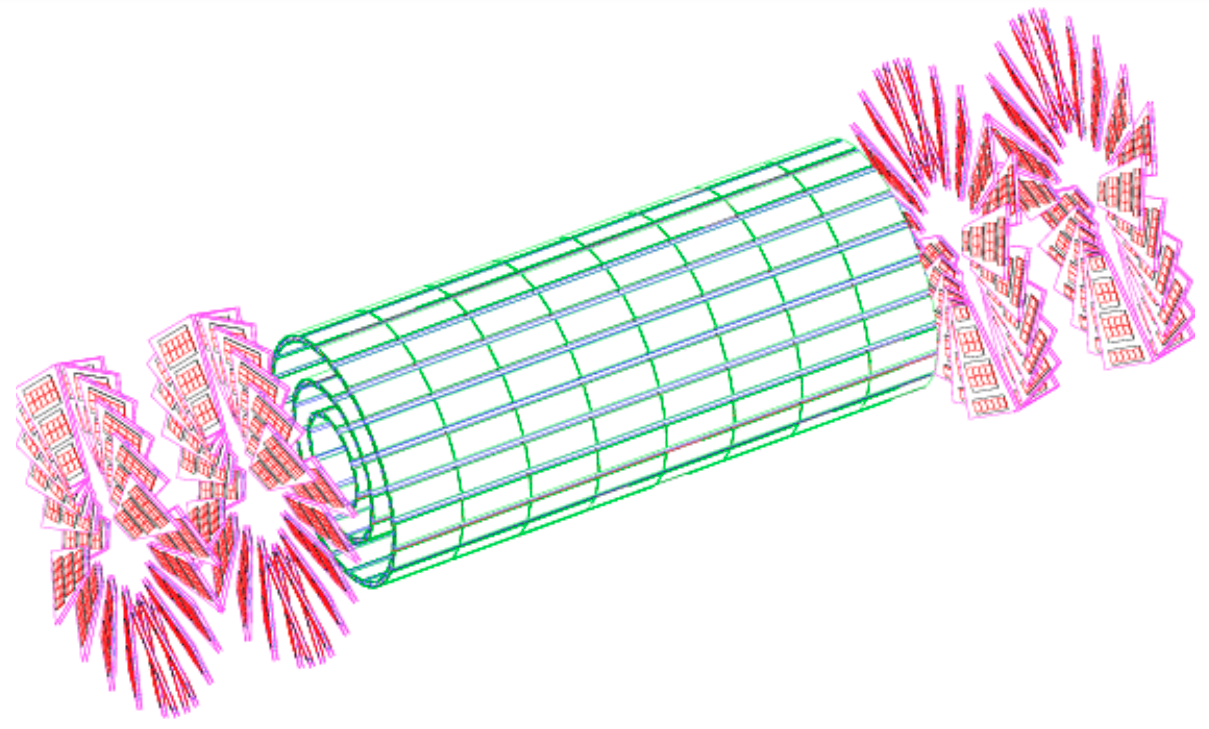
\includegraphics[width=0.50\textwidth]{figs/cms/tracker.png}
    \caption{Illustration of the pixel tracking layers. Note that this is the original layout;
      after the phase-1 upgrade in 2017, there is an additional layer in both the barrel
      and endcap systems. The pixel detector is 16 cm in radius and 100 cm long. (Image from~\cite{CMS:tdr_i})
            }
    \label{fig:cms_tracker}
  \end{center}
\end{figure}

The tracker consists of two main sub-modules. The first called the pixel detector, 
is close to the beamline and consists of arrays of 100 $\mu$m $\times$ 150 $\mu$m
silicon pixels, with 124 million pixels in total.
There are four barrel layers at radii 2.9, 6.8, 10.9, and 16.0 cm,
and three endcap layers. The detector provides coverage out to $|\eta|<2.4$.
The small size of the pixels allows for highly accurate identification of particle location.
An illustration of the pixel detector layout (before the 2017 phase-1 upgrade, which added
additional layers to the barrel and endcap) is shown in Fig.~\ref{fig:cms_tracker}.



\subsection{Electromagnetic calorimeter}
\subsection{Hadronic calorimeter}
\subsection{Muon detectors}
\subsection{Trigger system}
\subsection{Computing and reconstruction pipeline}


\section{Phase-2 CMS MIP timing detector}
